\documentclass[10pt,a4paper]{article}
\usepackage[margin=1.8cm,top=1.5cm,bottom=1.7cm]{geometry}
\usepackage[T1]{fontenc}
\IfFileExists{lmodern.sty}{\usepackage{lmodern}}{\usepackage{mathptmx}}
\usepackage{microtype,booktabs,graphicx,xcolor,tabularx,amsmath,enumitem}
\usepackage[font=small,labelfont=bf,skip=3pt]{caption}
\usepackage{float,placeins}
\usepackage{tikz}
\usetikzlibrary{positioning,arrows.meta,fit,backgrounds}
\usepackage[colorlinks,urlcolor=blue!60!black,linkcolor=black,citecolor=black]{hyperref}
\setlist{nosep,leftmargin=1.2em}
\setlength{\parskip}{2pt}
\setlength{\parindent}{0pt}
\setlength{\textfloatsep}{6pt}
\setlength{\floatsep}{5pt}
\setlength{\intextsep}{5pt}

% ---------------------------------------------------------------------------- set these
\newcommand{\repourl}{\textcolor{red}{https://github.com/TODO/bm25-vs-neural}}  % <-- your GitHub repository
% --------------------------------------------------------------------------------------
\IfFileExists{tables/macros.tex}{% generated by scripts/make_report_macros.py - do not edit
\newcommand{\corpusN}{\textcolor{red}{??}}
\newcommand{\corpusPrimary}{\textcolor{red}{??}}
\newcommand{\corpusInCat}{\textcolor{red}{??}}
\newcommand{\corpusFiltered}{\textcolor{red}{??}}
\newcommand{\corpusDup}{\textcolor{red}{??}}
\newcommand{\corpusWithdrawn}{\textcolor{red}{??}}
\newcommand{\corpusSha}{\textcolor{red}{??}}
\newcommand{\sciDiff}{\textcolor{red}{??}}
\newcommand{\sciOverlap}{\textcolor{red}{??}}
\newcommand{\sciCritI}{\textcolor{red}{??}}
\newcommand{\sciCritII}{\textcolor{red}{??}}
\newcommand{\sciPys}{\textcolor{red}{??}}
\newcommand{\sciBMplain}{\textcolor{red}{??}}
\newcommand{\sciBM}{\textcolor{red}{??}}
\newcommand{\sciEfive}{\textcolor{red}{??}}
\newcommand{\sciSpec}{\textcolor{red}{??}}
\newcommand{\sciHybE}{\textcolor{red}{??}}
\newcommand{\sciHybS}{\textcolor{red}{??}}
\newcommand{\reuDiff}{-0.0026}
\newcommand{\reuOverlap}{96.8}
\newcommand{\reuRatio}{1.900}
\newcommand{\reuDocs}{10{,}788}
\newcommand{\reuQueries}{100}
\newcommand{\truncEfive}{\textcolor{red}{??}}
\newcommand{\encMinEfive}{\textcolor{red}{??}}
\newcommand{\medTokEfive}{\textcolor{red}{??}}
\newcommand{\truncSpec}{\textcolor{red}{??}}
\newcommand{\encMinSpec}{\textcolor{red}{??}}
\newcommand{\medTokSpec}{\textcolor{red}{??}}
\newcommand{\gpuName}{\textcolor{red}{??}}
\newcommand{\bmIndexSec}{\textcolor{red}{??}}
\newcommand{\bmIndexMB}{\textcolor{red}{??}}
\newcommand{\bmMs}{\textcolor{red}{??}}
\newcommand{\bmVocab}{\textcolor{red}{??}}
\newcommand{\poolSize}{\textcolor{red}{??}}
\newcommand{\poolPerQ}{\textcolor{red}{??}}
\newcommand{\poolPrio}{\textcolor{red}{??}}
\newcommand{\anchorsFound}{\textcolor{red}{??}}
\newcommand{\anchorsMissing}{\textcolor{red}{??}}
\newcommand{\kappaLin}{\textcolor{red}{??}}
\newcommand{\kappaQuad}{\textcolor{red}{??}}
\newcommand{\nDouble}{\textcolor{red}{??}}
\newcommand{\ovBE}{\textcolor{red}{??}}
\newcommand{\ovBEId}{\textcolor{red}{??}}
\newcommand{\ovBEPara}{\textcolor{red}{??}}
\newcommand{\ovBS}{\textcolor{red}{??}}
\newcommand{\ovBSId}{\textcolor{red}{??}}
\newcommand{\ovBSPara}{\textcolor{red}{??}}
\newcommand{\ovES}{\textcolor{red}{??}}
\newcommand{\ovESId}{\textcolor{red}{??}}
\newcommand{\ovESPara}{\textcolor{red}{??}}
}{}
\newcommand{\inputor}[2]{\IfFileExists{#1}{\input{#1}}{#2}}
\newcommand{\pending}[1]{\textcolor{red!70!black}{[#1]}}
\newcommand{\st}[1]{\textsf{\small #1}}

\begin{document}
\begin{center}
{\Large\bfseries Domain-Specific Search: BM25 vs.\ Neural Retrieval on Technical Documents}\\[2pt]
{\large Intermediate Status Update \;|\; Information Retrieval \;|\; Group 10 \;|\; 25 October 2026}\\[4pt]
\begin{tabular}{llll}
Surajsinh Patil & 2025H1030058P & Tejas Mahajan & 2025H1030057P\\
Swayam Kumud & 2025H1030063P & Saksham Singhal & 2025H1030208P
\end{tabular}\\[3pt]
\textbf{Repository:} \repourl
\end{center}

% ======================================================================================
\section{Implementation status and architecture}
We compare our own BM25 implementation with two dense retrievers used without fine-tuning
(E5-base-v2 and SPECTER2) and their Reciprocal Rank Fusion hybrids on a frozen corpus of
\corpusN{} arXiv cs.CR abstracts, using 50 queries in five categories (exact identifier,
homonym, negation, time constraint, paraphrase). The whole pipeline is implemented, unit-tested
and runs end to end; Table~\ref{tab:status} lists the components.

\begin{table}[H]
\centering\small
\caption{Components built so far versus pending. Every built component has unit tests
(23 tests: BM25 against the formula, metrics against \texttt{pytrec\_eval}, kappa against scikit-learn, fusion, pooling).}
\label{tab:status}
\begin{tabularx}{\linewidth}{@{}l l X@{}}
\toprule
Component & Status & Notes\\
\midrule
Corpus builder (\texttt{corpus.py}) & done, frozen & \corpusN{} docs, SHA-256 \texttt{\corpusSha}; arXiv id list committed\\
Identifier-aware tokeniser + BM25 & done, validated & SciPy sparse matrix, vectorised scoring; matches Lucene (Sec.~\ref{sec:val})\\
Dense encoders + exact search & done & E5 (mean pooling, prefixes), SPECTER2 (proximity / ad-hoc query adapters)\\
RRF hybrids ($k{=}60$) & done & BM25+E5, BM25+SPECTER2 over top-100\\
Metrics, significance, CIs & done, validated & nDCG, P, MRR, MAP, R, Hole@10; permutation test + Holm; bootstrap CIs\\
Query set (50 + 5 practice) & done & TREC format; \anchorsFound{} anchors confirmed in corpus, \anchorsMissing{} being confirmed\\
Pooling + blind judging tool & done & \poolSize{} pairs ($\approx$\poolPerQ{}/query), 2 judges/query, offline HTML page\\
All five runs on cs.CR and SciFact & done & Kaggle T4 GPU; TREC run files and time/memory logs in the repository\\
Relevance judging & \textbf{in progress} & pages generated; phase 1 (any run's top-5, \poolPrio{} pairs) first \pending{update}\\
Evaluation on cs.CR, k1/b sweep, ablation & code done & run end to end; waiting for the frozen qrels\\
Stretch S1, S2 & runs done & cross-encoder and date-filtered runs produced; their new documents need judging\\
Stretch S3, S4 & code done & LLM judge, CC fusion (need qrels)\\
\bottomrule
\end{tabularx}
\end{table}

\textbf{Changes from the proposal.}
(1) The Pyserini check builds a Lucene index from exactly the same title+abstract text, so the
two BM25s differ only in the implementation.
(2) E5 is run through \texttt{transformers} with our own mean pooling, because
\texttt{sentence-transformers} and the \texttt{adapters} library needed by SPECTER2 require
incompatible library versions; a test checks the pooling against a manual computation.
(3) Besides validating BM25 on SciFact we run \emph{all five} systems there, which gives
judged results before our own judgments are finished.
(4) A judgment-free analysis of top-10 overlap between systems was added.
(5) For S2 we first use a rule-based date extractor (no API cost); the LLM extractor is optional.
(6) The filtered collection has fewer than the planned 50{,}000 documents, so it is used in full (no sampling).
Figure~\ref{fig:arch} shows the updated architecture.

\begin{figure}[h]
\centering
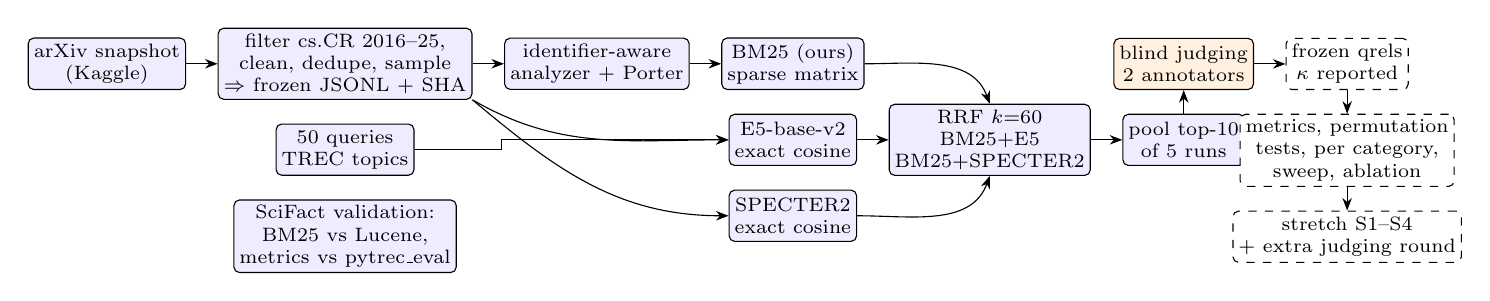
\begin{tikzpicture}[font=\scriptsize, node distance=3mm and 4mm,
  box/.style={draw, rounded corners=2pt, align=center, minimum height=6.5mm, fill=white, inner sep=2pt},
  done/.style={box, fill=blue!7}, todo/.style={box, dashed},
  arr/.style={-{Stealth[length=1.6mm]}, thin}]
\node[done] (snap) {arXiv snapshot\\(Kaggle)};
\node[done, right=of snap] (corp) {filter cs.CR 2016--25,\\clean, dedupe, sample\\$\Rightarrow$ frozen JSONL + SHA};
\node[done, right=of corp] (tok) {identifier-aware\\analyzer + Porter};
\node[done, right=of tok] (bm) {BM25 (ours)\\sparse matrix};
\node[done, below=of bm] (e5) {E5-base-v2\\exact cosine};
\node[done, below=of e5] (sp) {SPECTER2\\exact cosine};
\node[done, right=of e5] (rrf) {RRF $k{=}60$\\BM25+E5\\BM25+SPECTER2};
\node[done, right=of rrf] (pool) {pool top-10\\of 5 runs};
\node[box, fill=orange!12, above=of pool] (judge) {blind judging\\2 annotators};
\node[todo, right=of judge] (qrels) {frozen qrels\\$\kappa$ reported};
\node[todo, below=of qrels] (eval) {metrics, permutation\\tests, per category,\\sweep, ablation};
\node[todo, below=of eval] (str) {stretch S1--S4\\+ extra judging round};
\node[done, below=of corp] (q) {50 queries\\TREC topics};
\node[done, below=of q] (val) {SciFact validation:\\BM25 vs Lucene,\\metrics vs pytrec\_eval};
\draw[arr] (snap)--(corp); \draw[arr] (corp)--(tok); \draw[arr] (tok)--(bm);
\draw[arr] (corp.south east) to[out=-30,in=180] (e5.west); \draw[arr] (corp.south east) to[out=-40,in=180] (sp.west);
\draw[arr] (bm.east) to[out=0,in=110] (rrf.north); \draw[arr] (e5)--(rrf); \draw[arr] (sp.east) to[out=0,in=-110] (rrf.south);
\draw[arr] (rrf)--(pool); \draw[arr] (pool)--(judge); \draw[arr] (judge)--(qrels); \draw[arr] (qrels)--(eval); \draw[arr] (eval)--(str);
\draw[arr] (q.east) -- ++(1.1,0) |- (e5.west);
\end{tikzpicture}
\caption{Updated architecture. Shaded = implemented and run; orange = in progress; dashed = code
written and tested, waiting for the frozen qrels. Each stage is frozen before the next starts.}
\label{fig:arch}
\end{figure}

% ======================================================================================
\section{IR pipeline details}
\textbf{Corpus and preprocessing.} From the Kaggle arXiv snapshot we keep papers with cs.CR as
primary or cross-listed category and a first version in 2016--2025, remove withdrawn papers
(\corpusWithdrawn{}) and duplicate titles (\corpusDup{}), strip LaTeX and apply NFKC normalisation.
Of \corpusInCat{} cs.CR records in the snapshot, \corpusN{} remain and all are used
(\corpusPrimary{} with cs.CR as primary category). A document is its title plus abstract.

\textbf{BM25 (lexical).} The identifier-aware analyzer lower-cases, joins protocol versions
(``TLS v1.3'' $\to$ \texttt{tls1.3}), keeps identifiers such as \texttt{cve-2021-44228},
\texttt{sha-256} or \texttt{x86-64} as single unstemmed tokens and also indexes their parts,
which do not count towards document length (like Lucene's overlapping tokens). Other words
pass through Lucene's 33 English stopwords and the Porter stemmer. Note that ``no'' and ``not''
are stopwords, so BM25 cannot see negation at all. Term frequencies are stored once in a SciPy
CSC matrix (\bmVocab{} terms); for given $(k_1,b)$ the whole BM25-weighted matrix is computed in
one vectorised step with the Lucene IDF $\ln(1+\frac{N-n_t+0.5}{n_t+0.5})$, and a query is
scored with one sparse matrix--vector product. The main run uses $k_1{=}1.2$, $b{=}0.75$.

\textbf{Dense retrieval.} Both models are BERT-base (768 dimensions), used as published.
E5 uses the \texttt{query:}/\texttt{passage:} prefixes and mean pooling; SPECTER2 encodes
``title [SEP] abstract'' with its proximity adapter and queries with its ad-hoc query adapter
([CLS] vector). Documents are sorted by length for batching (fp16 on a \gpuName{}). Truncation is not an issue:
arXiv limits abstracts to 1{,}920 characters, the median document has \medTokEfive{} tokens and
fewer than 0.1\% exceed the 512-token limit.
Embeddings are cached and searched exactly (brute-force cosine), so no ANN approximation error
enters the comparison. \textbf{Hybrids} use RRF ($k{=}60$, fixed beforehand) over the top-100 of
each run, so no score normalisation and no tuning on our queries is needed.

\textbf{Judging and evaluation.} The top-10 of all five runs is pooled. Each query goes to two
of the four annotators (25 queries, $\approx$\,750 judgments each, every annotator pair shares
queries so $\kappa$ covers all pairs). The judging page shows documents in random order with no
system or rank, shows dates only for time queries, saves progress in the browser and exports JSON.
Disagreements are listed for an adjudication meeting and the qrels are then frozen with a checksum.
Metrics follow \texttt{trec\_eval} conventions (ties broken by docid, unjudged = non-relevant,
binary metrics at grade $\geq 2$). Significance: paired randomisation test (100k permutations,
exact enumeration for $n\leq 16$) with Holm--Bonferroni; per-category means get 95\% bootstrap CIs.

% ======================================================================================
\section{Preliminary evaluation results}\label{sec:val}
\textbf{Validation (success criteria i and ii).} On BEIR SciFact with identical settings
($k_1{=}0.9$, $b{=}0.4$, Lucene-like analyzer) our BM25 differs from Pyserini by
$\Delta$nDCG@10 $=$ \sciDiff{} (criterion~i \sciCritI{}, threshold 0.01) and shares
\sciOverlap\% of its top-10 documents. Our metric code reproduces \texttt{pytrec\_eval} on every
run and query (criterion~ii \sciCritII{}). The same check on an offline \reuDocs-document
collection gave $\Delta$nDCG@10 $=$ \reuDiff{}, \reuOverlap\% top-10 overlap, and a score ratio
of \reuRatio{} to Lucene, i.e.\ exactly the constant $(k_1{+}1)$ that Lucene omits; the small
remaining differences come from Lucene's lossy encoding of document length.

\inputor{tables/scifact.tex}{\begin{table}[h]\centering\small\caption{BEIR SciFact results.}\label{tab:scifact}
\pending{generated by \texttt{scripts/validate\_scifact.py --dense} (Kaggle notebook, section 2)}\end{table}}

\textbf{First comparison against the BM25 baseline (SciFact, 300 queries).}
E5 beats BM25 by +0.050 nDCG@10 ($p_{\text{Holm}}$ = \sciPBmtwofiveEfive; better on \sciWinEfive{}
queries, worse on \sciLossEfive{}), while SPECTER2 is 0.031 \emph{below} BM25 (not significant,
$p_{\text{Holm}}$ = \sciPBmtwofiveSpectertwo) and clearly below E5 ($p_{\text{Holm}}$ \sciPEfiveSpectertwo).
BM25+E5 is the best system (\sciHybE), significantly better than BM25 but not than E5 alone
(+0.014, $p_{\text{Holm}}$ = \sciPEfiveBmtwofiveEfive); its main effect is robustness: it is worse than
BM25 on only \sciLossHybE{} queries versus \sciLossEfive{} for E5. BM25+SPECTER2 is significantly
better than both of its components. So on SciFact the answers are RQ1 yes for E5 only, RQ3 no
(the general model wins), RQ4 partly. SciFact queries are natural-language claims, which favours dense
models; our identifier, negation and time queries test whether this holds on cs.CR.
\inputor{tables/scifact_significance.tex}{}

\textbf{cs.CR collection, no judgments needed.} Table~\ref{tab:overlap} shows that the systems
retrieve very different documents. BM25 and E5 share \ovBE{} of their top-10 on average, from
0.51 on homonym and \ovBEId{} on identifier queries down to \ovBEPara{} on paraphrases; SPECTER2
overlaps little with either. The near-disjoint lists on paraphrases are what we expected, and they
mean the hybrid always has complementary candidates. For the ten time queries we can already
count, from the first-version date, how many top-10 results break the date condition: 38\% for
BM25, 32\% for E5, 30\% for SPECTER2, 35\% for both hybrids and 31\% after cross-encoder
re-ranking (S1). No system uses the condition; the S2 date filter brings this to 0\%. Whether that
raises nDCG depends on the remaining documents being relevant, which judging will show.
Efficiency (Table~\ref{tab:eff}): BM25 indexes the corpus in \bmIndexSec{}\,s on one CPU core into
\bmIndexMB{}\,MB and answers a query in \bmMs{}\,ms. Each dense index is 116\,MB (4$\times$ larger) and
takes about 3 minutes of T4 time to build. A dense query takes 17--30\,ms, mostly query encoding
(exact search over all vectors takes about 6\,ms). Cross-encoder re-ranking of 100 documents adds 456\,ms per query.
\IfFileExists{tables/main_results-prelim.tex}{%
\textbf{Preliminary cs.CR results.} Table~\ref{tab:main-prelim} and Figure~\ref{fig:cat} use the
judgments exported so far, with disagreements resolved to the lower grade and unjudged documents
counted as non-relevant (see Hole@10). They are exploratory and will change once judging is
complete and adjudicated. \pending{One or two sentences on what they suggest, without claims of significance.}
\input{tables/main_results-prelim.tex}
\IfFileExists{figures/per_category-prelim.pdf}{\begin{figure}[t]\centering
\includegraphics[width=\linewidth]{figures/per_category-prelim.pdf}
\caption{Preliminary nDCG@10 per query category with 95\% bootstrap CIs (10 queries each; hatched = hybrids).}
\label{fig:cat}\end{figure}}{}}{}%
\inputor{tables/overlap.tex}{\begin{table}[h]\centering\small\caption{Top-10 overlap.}\label{tab:overlap}\pending{generated by \texttt{scripts/run\_overlap.py}}\end{table}}
\inputor{tables/efficiency_prelim.tex}{\begin{table}[h]\centering\small\caption{Efficiency.}\label{tab:eff}\pending{generated by \texttt{scripts/make\_report\_macros.py}}\end{table}}

% ======================================================================================
\FloatBarrier
\section{Path to final submission}\label{sec:path}
\begin{table}[H]
\centering\small
\caption{Plan for the remaining work (final submission mid-November).}
\begin{tabularx}{\linewidth}{@{}l X@{}}
\toprule
Dates & Work\\
\midrule
26--31 Oct & Finish judging (phase 2: ranks 6--10); compute $\kappa$ (target $\geq 0.6$, otherwise
revise guidelines and redo affected queries); adjudication meeting; freeze qrels.\\
1--4 Nov & Main results (RQ1, RQ3, RQ4) with significance tests; per-category analysis with CIs (RQ2);
k1/b sweep with 5-fold CV and tokenisation ablation (RQ5); check our pre-registered expectations.\\
5--9 Nov & Stretch goals S1 (cross-encoder re-ranking of the best run's top-100) and S2
(date filter on time queries); judge their new documents in an extra blind round.\\
9--12 Nov & Error analysis and case studies per category; S3/S4 if time allows.\\
12--15 Nov & Final report, figures, release code, queries, qrels and runs; demo preparation.\\
\bottomrule
\end{tabularx}
\end{table}
\textbf{Stretch objectives.} S1 and S2 have been run on cs.CR; S3 and S4 are implemented and tested
on synthetic data. \textbf{S1} re-ranks the top-100 of BM25+E5 with \texttt{ms-marco-MiniLM-L-6-v2}
(run done); we expect gains mainly on negation queries. \textbf{S2} parses the date range of each
time query (``after its 2018 standardisation'' $\to$ $\geq$2019; all 10 parsed correctly) and filters
on the first-version date (run done, removes 3.5 of the top-10 on average). The new documents these
runs bring into the top-10 will be judged blind in a second round once the main qrels are frozen. \textbf{S3} grades the same pool with an
LLM through any OpenAI-compatible endpoint and reports $\kappa$ and Kendall's $\tau$ of the system
ranking. \textbf{S4} tunes a convex combination of min-max normalised scores with stratified
5-fold CV. Order of priority is unchanged: S1, S2, then S3/S4.
\textbf{Risks.} Judging time (mitigated by phase-1 ordering); queries without a confirmed relevant
document (replaced via random abstracts, never via our systems); possible training-data overlap
of the dense models with arXiv abstracts (reported as a limitation).

% ======================================================================================
\section{Contribution matrix}
\begin{table}[H]
\centering\small
\begin{tabularx}{\linewidth}{@{}l X@{}}
\toprule
Member & Components owned and completed to date\\
\midrule
Surajsinh Patil & \pending{e.g.\ BM25 implementation, identifier-aware tokeniser, validation against Pyserini}\\
Tejas Mahajan & \pending{e.g.\ corpus builder and query set}\\
Swayam Kumud & \pending{e.g.\ dense encoders, GPU encoding, RRF}\\
Saksham Singhal & \pending{e.g.\ evaluation, significance tests, judging tool}\\
All & Query writing and review, relevance judging (two annotators per query)\\
\bottomrule
\end{tabularx}
\end{table}
\end{document}
